\documentclass[12pt]{article}
	
\usepackage[margin=1in]{geometry}		% For setting margins
\usepackage{amsmath}				% For Math
\usepackage{fancyhdr}				% For fancy header/footer
\usepackage{graphicx}				% For including figure/image
\usepackage{cancel}					% To use the slash to cancel out stuff in work
\usepackage[version=4]{mhchem}
\usepackage{tabularx}

\usepackage{chemfig}
\usepackage{endiagram}
\usepackage{booktabs}
\usetikzlibrary{tikzmark,positioning,shapes.geometric}
\definecolor{dullblue}{RGB}{178,201,231}


\newcommand\T{\rule{0pt}{5.0ex}}       % Top strut
\newcommand\B{\rule[-4.0ex]{0pt}{0pt}} % Bottom strut

%%%%%%%%%%%%%%%%%%%%%%
% Set up fancy header/footer
\pagestyle{fancy}
\fancyhead[LO,L]{Dr. Craig Waitt}
\fancyhead[CO,C]{Acid and Bases - Trine Teaching Demo}
\fancyhead[RO,R]{\today}
\fancyfoot[LO,L]{}
\fancyfoot[CO,C]{\thepage}
\fancyfoot[RO,R]{}
\renewcommand{\headrulewidth}{0.4pt}
\renewcommand{\footrulewidth}{0.4pt}
%%%%%%%%%%%%%%%%%%%%%%

\begin{document}
\section{Learning Objectives}
\begin{enumerate}
    \item How does water act as an acid or a base?
    \item What is the relationship between [\ce{H3O^{+}}] and [\ce{OH-}]?
    \item How do we measure the strength of an acid?
\end{enumerate}

\section{Recap}
\begin{enumerate}
    \item Acids and Bases share distinct physical and chemical properties.
    \begin{enumerate}
        \item Touch, taste, reaction with metals, etc.
    \end{enumerate}
    \item Different theories on how to define if a substance is an acid or base?
    
    \begin{center}
        \begin{tabularx}{0.8\textwidth}{| >{\centering\arraybackslash}X | >{\centering\arraybackslash}X | >{\centering\arraybackslash}X | >{\centering\arraybackslash}X |}
        \hline
        \textbf{Theory} & \textbf{Acid} & \textbf{Base} & \textbf{Notes} \T\B \\
        \hline
        Arrhenius \T & Produces \ce{H+} & Produces \ce{OH-} & Limited to aqueous solutions \B \\  
        \hline
        Brønsted \T & Donates \ce{H+} & Accepts \ce{H+}  & Acids must contain \ce{H+} \B \\  
        \hline
        Lewis \T & Accepts electrons & Donates electrons & Limited to transfer of a single electron \B \\  
        \hline
    \end{tabularx}
    \end{center}
    
    \item Within the Brønsted definition: we looked at how combining acids and bases create salt and water (neutralization reactions).

    \begin{align*}
    \ce{HCl(aq) + NaOH(aq) &<--> NaCl(aq) + H2O(l)} \\
    \ce{HCl(aq) + NaOH(aq) <-->& Na+(aq) + Cl-(aq) + H2O(l)} 
    \end{align*}

    \newpage 
    
    \item Within the Brønsted definition: we looked at determining conjugate acid-base pairs.

    \begin{figure}[h] 
	\begin{centering}
		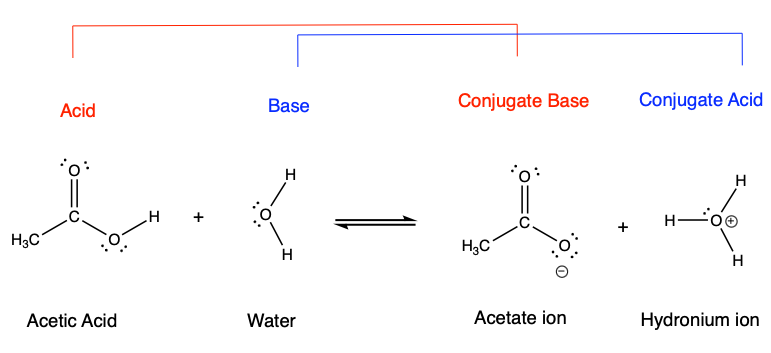
\includegraphics[width=\textwidth,trim={0 0 0 0cm},clip]{Figures/Conj-A-B-pairs-1.png}
	\end{centering}
    \end{figure}    


     \begin{figure}[h] 
	\begin{centering}
		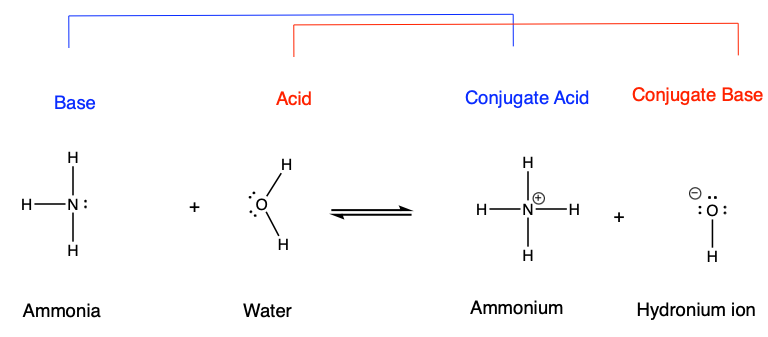
\includegraphics[width=\textwidth,trim={0 0 0 0cm},clip]{Figures/Conj-A-B-pairs-2.png}
	\end{centering}
    \end{figure}    
    
\end{enumerate}

\newpage

\section{Acid-Base Properties of Aqueous Solutions are Governed by the Autoionization of Water}

\noindent The previous example shows that water can act as an acid or a base according to the environment around it. On its own, water is a weak electrolyte but does undergo ionization to a small extent (as demonstrated below). This reaction is sometimes known as \textbf{autoionization of water}.

\begin{figure}[h] 
    \begin{centering}
	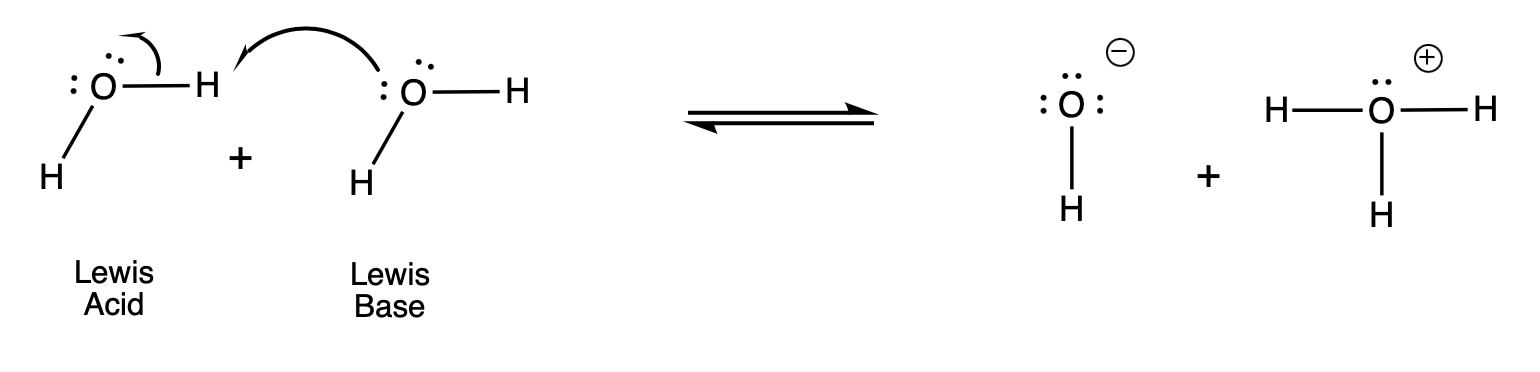
\includegraphics[width=\textwidth,trim={0 2cm 0 0},clip]{Figures/H2O-auto.png}
    \end{centering}
\end{figure}  


\noindent The reaction as written indicates that there is an equilibrium between liquid water (reactants) and the hydronium and hydroxide ions (products). Therefor, we can express the equilibrium constant for the autoionization of water:

\begin{equation}
    K = \frac{\alpha_{\ce{H3O+}}\alpha_{\ce{OH-}}}{\alpha_{\ce{H2O}}^{2}}
\end{equation}

\noindent Typically, the concentrations of \ce{H3O+} and \ce{OH-} are sufficiently small that their activities are to a good approximation equal to their molar concentrations. This means that $\alpha_{\ce{H3O+}} = [\ce{H3O+}]$, $\alpha_{\ce{OH-}} = [\ce{OH-}]$, and $\alpha_{\ce{H2O}} = 1$. As a result, our equilibrium constant above can be rewritten as:

\begin{equation}
    K_{w} = [\ce{H3O+}][\ce{OH-}] \\
\end{equation}
\noindent or
\begin{equation}
\label{eq:K_w_expression}
    K_{w} = [\ce{H+}][\ce{OH-}]
\end{equation}

\noindent  $K_{w}$ is known as the \textbf{ion-product constant} which is the product of the molar concentrations of \ce{H+} and \ce{OH-} ions at a particular temperature. It is important to note that $K_{w}$ (like all other equilibrium constants) is dimensionless. The actual expression (in terms of activity) is written as:

\begin{equation}
    K_{w} = \left[\frac{\ce{H3O+}}{c^{\circ}}\right]\left[\frac{\ce{OH-}}{c^{\circ}}\right]
\end{equation}

\noindent where $c^{\circ} = 1 M$. For simplicity $c^{\circ}$ is omitted from the $K_{w}$ expressions. Therefore, it is imperative to be careful to convert the concentration units to $M$ before using equation \ref{eq:K_w_expression}.
\\
\\
\noindent In pure water at $25^{\circ}\text{C}$, the concentration of \ce{H3O+} and \ce{OH-} are equal and found to be $[\ce{H+}] = [\ce{OH-}] = 1 \times 10^{-7} M$. This means that $K_{w}$ is:

\begin{equation}
    K_{w} = [\ce{H3O+}][\ce{OH-}] = [1 \times 10^{-7} M][1 \times 10^{-7} M] = 1.00 \times 10^{-14}
\end{equation}

\noindent \textbf{The value of $K_{w}$ is fixed at $25^{\circ}\text{C}$ regardless if we have a pure solution of water or an aqueous solution of dissolved species.} Now given an arbitrary solution, we can now determine how acidic or basic it is.

\subsection{Measuring the Acidity or Alkalinity of a Solution}

\noindent We can determine if a dilute solution is acidic or basic by measuring (or calculating) the relative concentration of \ce{H3O+} and \ce{OH-}.

\begin{center}
\begin{tabularx}{0.8\textwidth}{| >{\centering\arraybackslash}X | >{\centering\arraybackslash}X | }
    \hline
    $[\ce{H3O+}] > [\ce{OH-}]$ & Acidic  \T\B \\
    \hline
    $[\ce{H3O+}] < [\ce{OH-}]$ & Basic  \T\B \\
    \hline
    $[\ce{H3O+}] = [\ce{OH-}]$ & Neutral  \T\B \\
    \hline
\end{tabularx}
\end{center}

\noindent In practice, we can change the $[\ce{H3O+}]$ and $[\ce{OH-}]$, but we cannot vary them independently. If we adjust the solutions $[\ce{H3O+}]$, the $[\ce{OH-}]$ \textit{must} change to.

\subsubsection{Exercise}

The concentration of \ce{OH-} ions in certain household cleaning solutions is approximately $0.0025 M$. What is the concentration of \ce{H3O+} ions. Is the solution acidic, basic, or neutral?

\begin{align*}
    &\ce{H2O(l) + H2O(l) <--> H3O+(aq) + OH-(aq)} \\
    \\
    &K_{w} = [\ce{H3O+}][\ce{OH-}]\\
    \\
    &[\ce{H3O+}] = \frac{K_{w}}{[OH-]} \\
    \\
    &[\ce{H3O+}] = \frac{1.00 \times 10^{-14}}{0.0025} \\
    \\
    &[\ce{H3O+}] = 4 \times 10^{-12} 
\end{align*}
\indent The solution is basic because the concentration of $[\ce{OH-}] > [\ce{H3O+}].$


\newpage

\subsection{pH - a Measure of Acidity}

We typically deal with very small concentrations of $[\ce{H+}]$ and $[\ce{OH-}]$ ions. A more practical measure of acidity (and alkalinity) is called \textbf{pH}. The \textbf{pH} of a solution is defined as the \textit{negative logarithm (base 10) of the hydrogen ion activity}:

\begin{equation}
\text{pH} = -\log(\alpha_{\ce{H+}}) \quad \text{or} \quad  \text{pH} = -\log(\alpha_{\ce{H3O+}})
\end{equation}

\noindent Similarly as described in the previous section, for dilute solutions in which the hydrogen (and hydronium) ion concentrations can be well approximated by its concentration relative to standard concentration:

\begin{equation}
    \text{pH} = -\log(\alpha_{\ce{H+}}) \approx \text{pH} = -\log([\ce{H+}])
\end{equation}

\noindent Again, [\ce{H+}] typically has units on $M$, however, we ignore units for convenience. The pH of a solution is a dimensionless quantity. The equation above is simply designed to give a convenient number to work with.
\\
\\
\noindent Because pH is simply a way to express hydrogen ion concentration, acidic and basic solution can be identified based on their pH.
\\
\\
\noindent If a solution is neutral, that is equivalent as saying the concentrations of \ce{H3O+} = \ce{OH-}. With that, we can calculate the pH of a neutral solution.

\begin{align*}
    K_{w} &= [\ce{H3O+}][\ce{OH-}] = [\ce{H3O+}]^{2} \\
    \\
    [\ce{H3O+}] &= \sqrt{1.00 \times 10^{-14}} = 1.00 \times 10^{-7} \\
    \\
    \text{pH} &= -\log([\ce{H3O+}]) = -\log(1.00\times10^{-7}) = 7\\
\end{align*}

\noindent We can follow similar procedures for acidic solutions and basic solutions. The table below summarizes the conditions of a solution at $25^{\circ}$C.

\begin{center}
\begin{tabularx}{0.8\textwidth}{| >{\centering\arraybackslash}X | >{\centering\arraybackslash}X | >{\centering\arraybackslash}X |}
\hline
   & [\ce{H+}] & pH \T\B \\
 \hline
 Acidic	 & $> 1.00 \times 10^{-7}$ &  $< 7$ \T\B \\  
 \hline
 Basic  & $< 1.00 \times 10^{-7}$ &  $> 7$ \T\B \\
  \hline
 Neutral & $= 1.00 \times 10^{-7}$ &  $= 7$  \T\B \\
  \hline
\end{tabularx}
\end{center}

\subsubsection{Exercise}

The pH of rainwater collected in a region of the northeastern United States on a particular day was 4.82. Calculate the \ce{H3O+} and \ce{OH-} concentration of the rainwater.

\begin{align*}
        \text{pH} &= -\log([\ce{H3O+}]) \\
    \\
    [\ce{H3O+}] &= 10^{-\text{pH}} \\
    \\
    [\ce{H3O+}] &= 10^{-4.82} \\
    \\ 
    [\ce{H3O+}] &= 1.51 \times 10^{-5} \\
    \\
    K_{w} &= [\ce{H3O+}][\ce{OH-}] \\ 
    \\
    [\ce{OH-}] &= \frac{K_{w}}{[\ce{H3O+}]} = \frac{K_{w}}{10^{-\text{pH}}} \\
    \\
    [\ce{OH-}] &= \frac{1.00\times10^{-14}}{10^{-4.82}} = 6.61 \times 10^{-10} \\
\end{align*}

\newpage

\end{document}
